\section{Model Order Reduction on Solutions}
The underlying idea of MOR is that each high-dimensional solution can be represented in a low-fidelity space through a reduced number of global basis functions. By extracting the most significant features from high-dimensional datasets, MOR enables the creation of reduced-order models that retain essential dynamical behaviour on a reduced basis space. This approach proves particularly advantageous in scenarios where computational resources are limited or rapid simulations are required. There are many techniques for generating the reduced basis spaces, such as the Proper Orthogonal Decomposition (POD), the Proper Generalized Decomposition (PGD) and the Principle Component Analysis(PCA). In this project, we focused on using POD on the snapshot matrix to obtain the reduced basis space, and the Python RBniCSx package provided full support for the related operations in POD. 

\subsection{Proper Orthogonal Decomposition}

The appeal of POD lies in its ability to identify the dominant modes of variation in data through singular value decomposition (SVD). Singular value decomposition was performed to identify the most significant eigenvalues and their related eigenvectors. These eigenvectors form the reduced basis space, where the full-order solutions are projected.  

Consider a snapshot matrix $\mathbf{S}$ of dimension $N \times M$, where $N$ is the number of snapshots and M is the degrees of freedom for each high-fidelity FEM solution. By performing singular value decomposition (SVD) on $\mathbf{S}$, we can express $\mathbf{S}$ as:

\begin{equation}
    \mathbf{S} = \mathbf{U}\mathbf{\Sigma}\mathbf{V}^T
    \label{eqn:SVD}
\end{equation}

Where $\mathbf{U}$ is an $N \times N$ matrix containing the left singular vectors (also known as POD modes or basis functions), $\mathbf{\Sigma}$ is the $N \times M$ diagonal matrix containing the singular values $\{\sigma_1, \sigma_2,...,\sigma_{min(N,M)}\}$ in decreasing order, and $\mathbf{V}^T$ is the transpose of an $M \times M$ matrix containing the right singular vectors.

If we want to obtain the $L$ basis functions $\mathbf{u_{rb}} = \{\mathbf{u}_1,...,\mathbf{u}_L\}$ that best represent the snapshot matrix $\mathbf{S}$, we would pick the left eigenvectors in $\mathbf{U}$ corresponding to the most significant $L$ singular values from $\mathbf{\Sigma}$ (i.e. $\{\sigma_1, \sigma_2,...,\sigma_{L}\}$). 

We can reinforce two stopping criteria to determine the value of $L$ (i.e., the number of modes that form the reduced basis space). The first one is to set an arbitrary maximum number of modes $N_{max}$ that we are willing to accept. The second criterion is the tolerance on the retained energy $\epsilon$. This is defined as the ratio between the smallest singular value to the largest singular value (i.e. pick $L$ such that $\epsilon \geq \frac{\sigma_{L}}{\sigma_1}$). In practice, we will stop when either condition is met.

\subsection{Solution Projection}
Once we have the modes, we have formed the reduced basis space $\mathbf{V}_{rb}$ where each FEM solution can then be projected. To project a high-fidelity solution $\mathbf{s}$ onto a reduced basis space represented by $\mathbf{u_{rb}} = \{\mathbf{u}_1,...,\mathbf{u}_L\}$, we can use the Galerkin projection method. This involves computing the inner product of the high-fidelity solution with each basis function and multiplying it by the corresponding basis function. Mathematically, this is given by: 

\begin{equation*}
    \mathbf{s}_{rb} = \sum_{i=1}^{L} \langle \mathbf{s}, \mathbf{u}_i \rangle  \mathbf{u}_i
\end{equation*}

Where the operation $\langle \mathbf{s}, \mathbf{u}_i \rangle$ defines the inner production action between the high-fidelity solution and the $i^{th}$ basis function.  

\subsection{Solution Reconstruction}

Later in the report, we will discuss the use of ANN in obtaining the predicted solutions on the reduced basis space. However, we are still interested in the full-order solution, which requires a way of reconstructing the high-fidelity solution and measuring the error between the original FEM solution and the reconstructed solution. For a set of basis functions $\mathbf{u_{rb}} = \{\mathbf{u}_1,...,\mathbf{u}_L\}$ and a reduced basis solution $\mathbf{s}_{rb} = \{s_1,...,s_L\}$, the reconstructed solution $\mathbf{v}$ can be simply represented by multiplying the basis functions by their corresponding coefficients and summing over all modes:

\begin{equation}
    \mathbf{v} = \sum_{i=1}^{L} s_i \cdot \mathbf{w}_i 
    \label{eqn:reconstruction}
\end{equation}

To measure the error between the original solution and the reconstructed solution, the relative error was calculated as the $L_2$-norm of the error the to $L_2$-norm of the original solution $\mathbf{u}$, which would give us a percentage that represents the amount of deviation from the FEM solution:

\begin{equation}
   \epsilon = \frac{\| \mathbf{u} - \mathbf{v} \|}{\| \mathbf{u} \|}
   \label{eqn:norm_error}
\end{equation}

The specific norm operation is defined by the specific definition of the inner product action used in the function. The $L_2$-norm is commonly used in functional analysis and finite element methods to measure the magnitude of functions, which is defined in equation \ref{eqn:L2norm}. 

\begin{equation}
    \| f \|_{L_2(\Omega)} = \left( \int_{\Omega} |f(x)| |q(x)| \, dx \right)^{1/2}
    \label{eqn:L2norm}
\end{equation}

The other possible choice is the $H_1$-norm that incorporates the first derivative of the function given by equation \ref{eqn:H1norm}. The $H_1$-norm would incur additional computational cost in computing the gradient term. In this report, we used the $L_2$-norm inner product action for $u$ because it provides a measure of magnitude without considering directional information. 

\begin{equation}
    \| f \|_{H_1(\Omega)} = \left( \| f \|_{L_2(\Omega)}^2 + \| \nabla f \|_{L_2(\Omega)}^2 \right)^{1/2}
    \label{eqn:H1norm}
\end{equation}

For the case of $\sigma$, we included the inner product of the divergence term in the $L_2$-norm. This is similar to equation \ref{eqn:H1norm}, but changed the grad operation to divergence due to $\sigma$ being a vector field, as shown in equation 
\ref{eqn:sigma_norm}. This also helps to capture the spatial variation (i.e. the smoothness) of the fields. 

\begin{equation}
    \| f \| = \left( \| f \|_{L_2(\Omega)}^2 + \| \nabla \cdot f \|_{L_2(\Omega)}^2 \right)^{1/2}
    \label{eqn:sigma_norm}
\end{equation}

\textcolor{red}{Hopefully correct inner product}



\subsection{Choice of Parameters based on POD Result}
In Section 3, an examination was conducted regarding the selection of parameters ($\bm{\mu}=[\mu_1, \mu_2]$ versus $\bm{\mu} = [\mu_1, \mu_2, \mu_3, \mu_4, \mu_5]$), and we explained our rationale in using only 2 parameters by showing the large variability of the solution manifold imposed by changing 5 parameters altogether. Over here, we will provide a more quantitative justification by contrasting the Proper Orthogonal Decomposition (POD) outcomes obtained using different parameterisations. 

Each parameter is adjusted along a Numpy \textit{linspace} scale, ensuring equal intervals between values. Combining each value creates a collection of input parameters. The full-order model was solved for each $\bm{\mu}$, followed by performing POD on the snapshot matrix, which creates a reduced basis space. In the first case, we only varied the two parameters $\mu_1$ and $\mu_2$, each taking 10 values (a total of 100 solutions for POD). In the second case, we varied all 5 parameters taking $4 \times 4 \times 3 \times 3 \times 3$ values (a total of 432 solutions for POD). In both cases, we set $N_{max} = 20$ and $\epsilon = 10^{-4}$ as the stopping criterion \footnote{see Section 4.1 for details}.

\begin{figure}[!h]
    \centering
    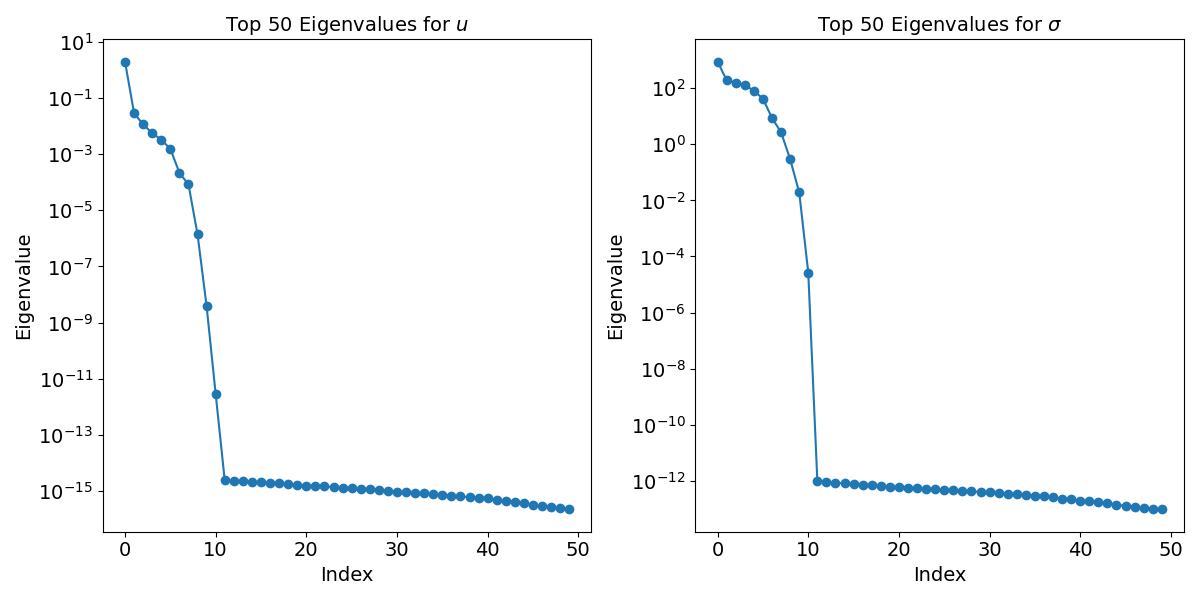
\includegraphics[width=0.8\linewidth]{fig_pod/eigendecay_10,10.png}
    \caption{Top 50 Eigenvalues from POD with varying $\mu_1$ and $\mu_2$, each parameter spanning 10 discrete values}
    \label{fig:eigendecay_10by10}
\end{figure}

\begin{figure}[!h]
    \centering
    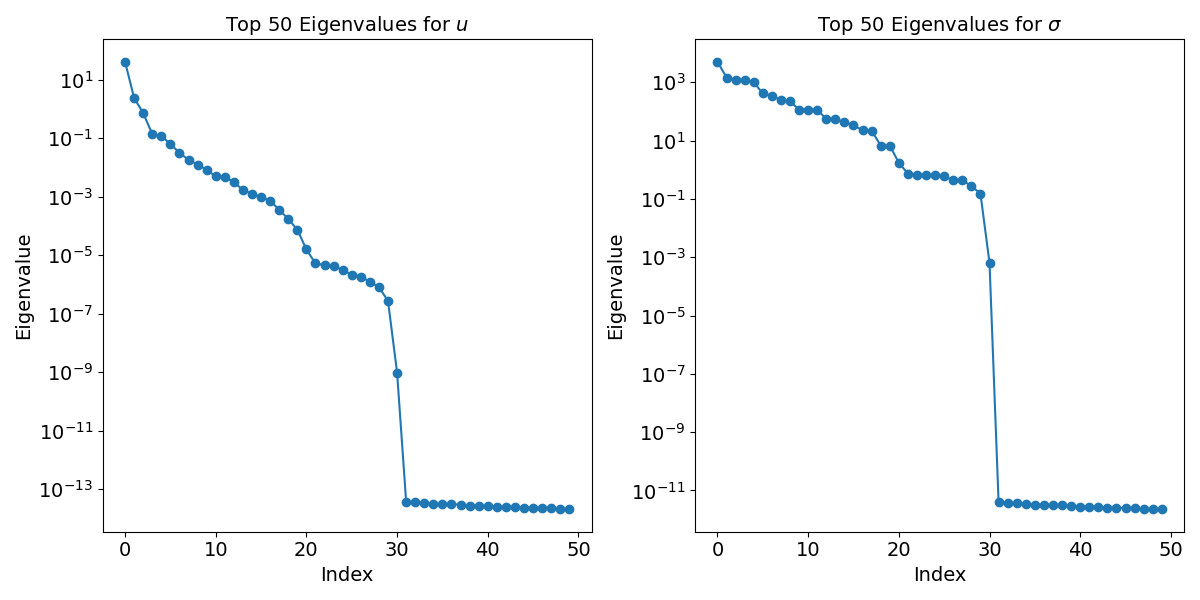
\includegraphics[width=0.8\linewidth]{fig_pod/eigendecay_4,4,3,3,3.png}
    \caption{Top 50 Eigenvalues from POD with varying all parameters, with $\mu_1$ and $\mu_2$ spanning 4 discrete values and the rest spanning 3 discrete values}
    \label{fig:eigendecay_allvary}
\end{figure}

To measure the accuracy and reliability of POD, we initialised 100 random samples of input parameters and solved for the high-fidelity solutions using FEM. The solutions were then projected onto $\mathbf{V}_{rb}$ with $\mathbf{u}_{rb}$ to form the reduced basis solution $\mathbf{s}_{rb}$. The quality of POD can then be quantified by calculating the average relative error of the solution reconstructed using equation \ref{eqn:reconstruction} and \ref{eqn:norm_error}. Table \ref{tab:POD_results} compares the proposed two cases, where we can observe that the reconstruction error for both $u$ and $\sigma$  were greatly reduced with only 2 parameters, as well as the size of the reduced basis space. Note that for $\sigma$ in the 5-parameter case, the size of the reduced basis was even reaching the maximum threshold $N_max$, meaning that ideally we still need more modes to capture the features of the solutions. Getting the POD error as small as possible is an essential first step in the project. Only with a reasonably accurate POD process can we safely proceed to the next step of ANN training. 

\begin{table}[htb]
    \centering
    \caption{Results of POD reconstruction relative error on different parameter sets}
    \small
    \begin{tabular}{c|c|c|c|c}
        \toprule
        Parameters & Sample Size & Size of $\mathbf{V}_{rb}$ ($u$, $\sigma$) & Mean Error ($u$, $\sigma$) & Max Error ($u$, $\sigma$) \\
        \midrule
        2 & $10 \times 10$ & (7, 9) & (0.012, 0.005) & (0.067, 0.015) \\
        5 & $4 \times 4 \times 3 \times 3 \times 3$ & (14,20) & (0.062, 0.246) & (0.293, 0.781)  \\
        \bottomrule
    \end{tabular}
    \label{tab:POD_results}
\end{table}

In addition to the relative error, we can compare eigenvalues obtained from SVD for different snapshot matrices. In general, if the eigenvalue decays faster, we can obtain a lower intrinsic dimensional space representing the parametric dependence on high-fidelity solutions. This would not only enhance the computational efficiency but also increase the accuracy of POD. Figure \ref{fig:eigendecay_10by10} shows the decay of eigenvalues when performing SVD on the snapshot matrix, varying $\mu_1$ and $\mu_2$, each parameter spanning 10 discrete values (total 100 combinations). Figure \ref{fig:eigendecay_allvary} shows the decay of eigenvalues when varying all parameters, with the number of values for $\bm{\mu}$ equals $[4,4,3,3,3]$ (total 432 combinations). The eigenvalues for both  $u$ and $\sigma$ decay very quickly with only 2 varying parameters, while taking slightly longer for the 5 parameter case. This also corresponds to the fact that a higher number of reduced basis functions was needed.  

Further to the accuracy of POD, the computational efficiency of the POD process is also greatly hindered by the high number of training snapshots needed with more parameters. Due to the nature of the snapshot matrix being a dense matrix, it was impossible to parallelise the process across multiple CPU cores, so the POD process would take a long time in serial. In addition, a higher number of reduced basis sizes would also incur additional costs in projecting the high-fidelity solution onto the reduced basis space. This proved to be particularly costly as we later tried to initialise the training inputs for the ANN, which required a large amount of data points.

\newpage